\paragraph{Analysis of representations}
In addition to evaluating the model via task performance metrics, we
analyze the spoken utterance embeddings. There are a variety of
methods typically applied to this task, such as variants of diagnostic
probing, and representational similarity analysis (RSA). We focus on
a generalization of the latter approach.
The classical RSA was developed to analyze brain imaging data
\citep{kriegeskorte2008representational} and adapted for probing
neural network representations
\citep[e.g.][]{chrupala-alishahi-2019-correlating}. The method
consists in computing pairwise similarity scores for stimuli (such as
utterances) in two representation spaces: one being the subject of
analysis (i.e.\ neural activation space) and the other the benchmark
representation space (e.g.\ syntax tree space). The strength of
correlation between the pairwise similarity scores in the two spaces
quantifies to what extent the benchmark representation is encoded in
the neural activation patterns. In the current work we generalize this
idea such that it becomes possible to relate
neural activation similarity space and several different factors that
we hypothesize may be associated with it. Namely, we treat the
similarity scores in the neural activation space as regression targets
and fit a linear model with a number of predictors which 
correspond to control variables or hypothesized relevant factors.

Specifically, we compute pairwise cosine similarities between
model-embedded one-word or multi-word utterances from our validation data: these are
the regression targets. The variables are listed in \Cref{tab:grsa-variables}.

\begin{table}
  \centering
  \begin{tabular}{lp{0.7\linewidth}}\toprule
    Name              & Meaning \\\midrule
    sim$_2$           & Cosine similarity between representations,
                        from fully trained model,
                        of two audio clips \\
    sim$_1$           & Cosine similarity between representations,
                        from pre-trained-only model,  of two audio
                        clips \\
    semsim            & Cosine similarity between summed GloVe word-type-embeddings for two clips\\
    sametype          & Two clips correspond with the same transcription \\
    samespeaker       & Two clips uttered by same speaker\\
    sameepisode       & Two clips are from the same episode\\
    durationdiff      & Absolute difference in duration between two
                        clips\\
    durationsum       & Sum of the duration of the two clips\\
  \end{tabular}
  \caption{Variable definitions for the multiple RSA analysis.}
  \label{tab:grsa-variables}
\end{table}

\todo{THIS IS NOT QUITE RIGHT: For this analysis, we exclude word pairs where either word is out of
vocabulary for the GloVe dataset.} In order to obtain model embeddings
for the utterances, we use forced-alignment of audio with
corresponding subtitles, discarding cases where alignment fails.
%For
%the dialog condition the number of pairwise scores for the remaining
%tokens is X; for the narration condition it is Y.

The coefficients of the regression model serve as the estimates of the
strength of the association of each predictor with the target variable
(pairwise similarity), while controlling for the other predictors. 



\paragraph{Multiple representational similarity analysis}

For the single-word setting, 
\Cref{tab:dialogvarcor} and \Cref{tab:narrationvarcor} show the raw
correlations between variables in the multiple RSA analysis, while
\Cref{fig:coef_word_dialog} and \Cref{fig:coef_word_narration} show the
standardized regression coefficients, where the target variable is
pairwise representation similarity for the pre-trained-only and the
fully-trained versions of the target model.



\begin{figure}
  \centering
  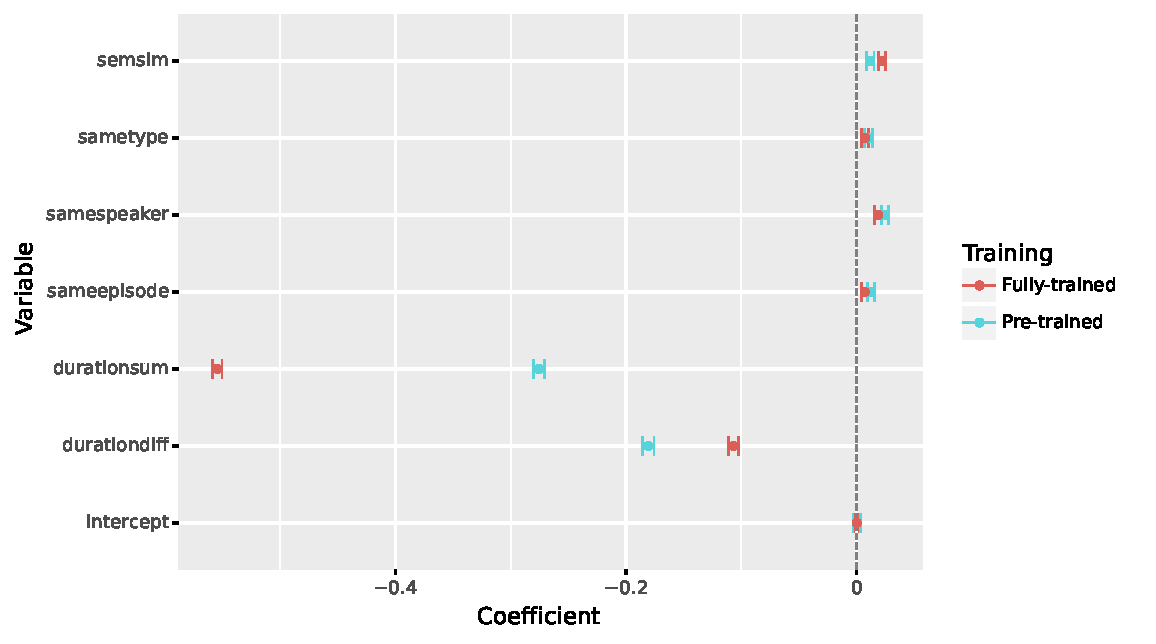
\includegraphics[scale=0.66]{results/grsa_dialog_word_coef.pdf}
  \caption{Association of predictors with trained and untrained
    model-based pairwise similarity scores for single-word utterances
    in the dialog validation data. Coefficients are standardized.}
  \label{fig:coef_word_dialog}
\end{figure}

\begin{figure}
  \centering
  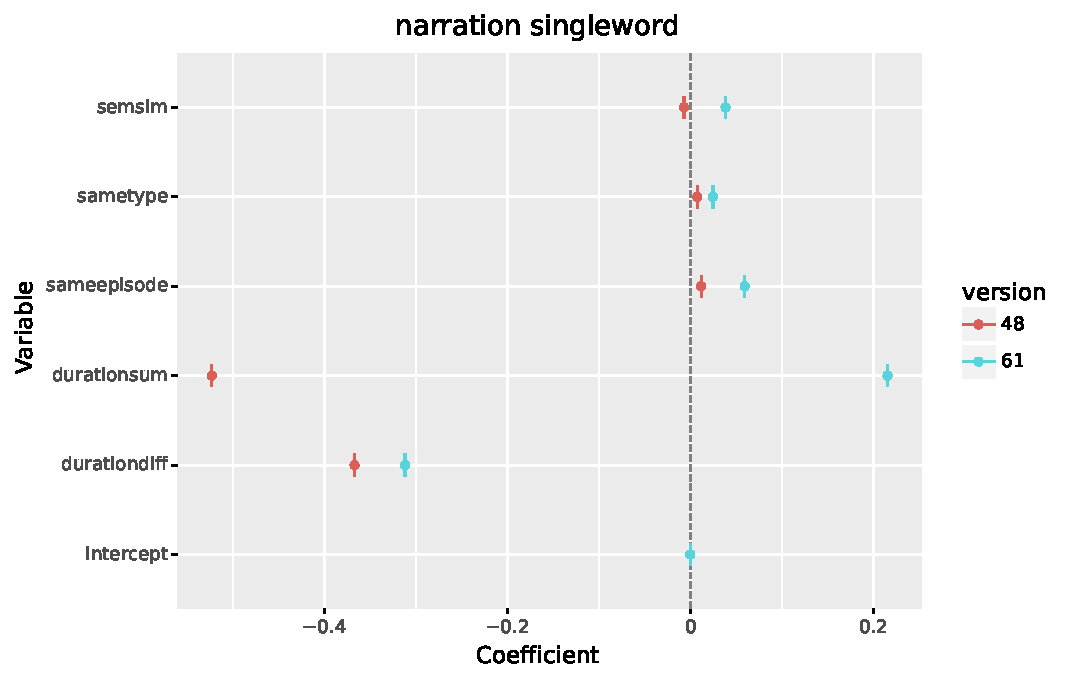
\includegraphics[scale=0.66]{results/grsa_narration_word_coef.pdf}
  \caption{Association of predictors with 
    model-based pairwise similarity scores for single-word utterances
    in the narration validation data. Coefficients are standardized.}
  \label{fig:coef_word_narration}
\end{figure}


For the multi-word setting, \Cref{fig:coef_multiword_dialog} and
\Cref{fig:coef_multiword_narration} show the regression coefficients.
\begin{figure}
  \centering
  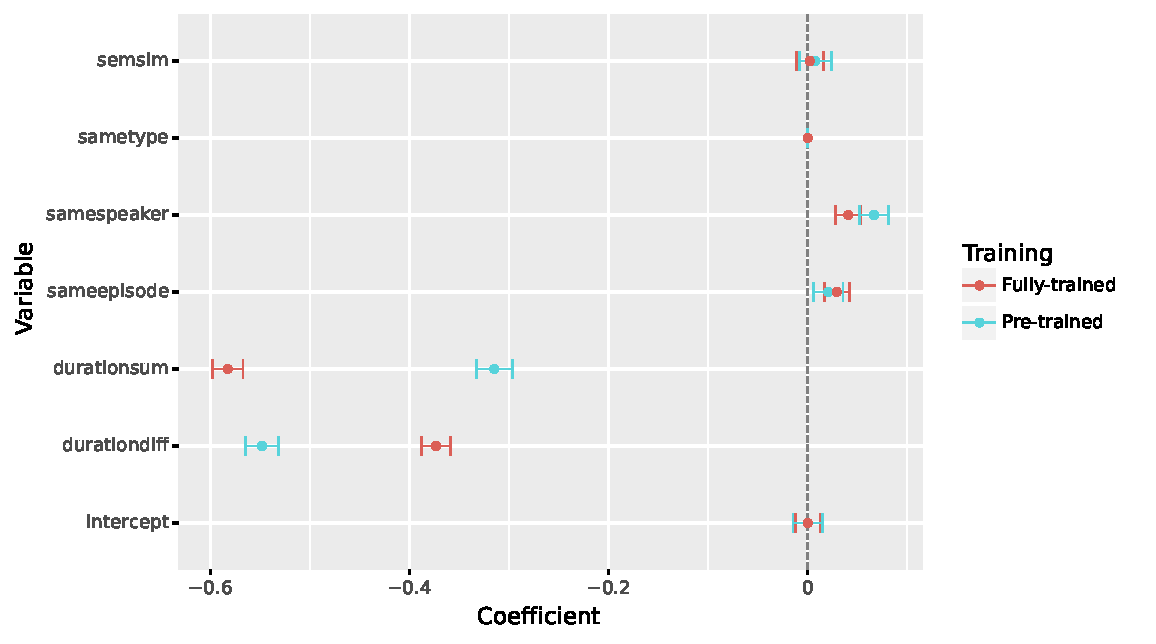
\includegraphics[scale=0.66]{results/grsa_dialog_multiword_coef.pdf}
  \caption{Association of predictors with 
    model-based pairwise similarity scores for multi-word utterances
    in the dialog validation data. Coefficients are standardized.}
  \label{fig:coef_multiword_dialog}
\end{figure}

\begin{figure}
  \centering
  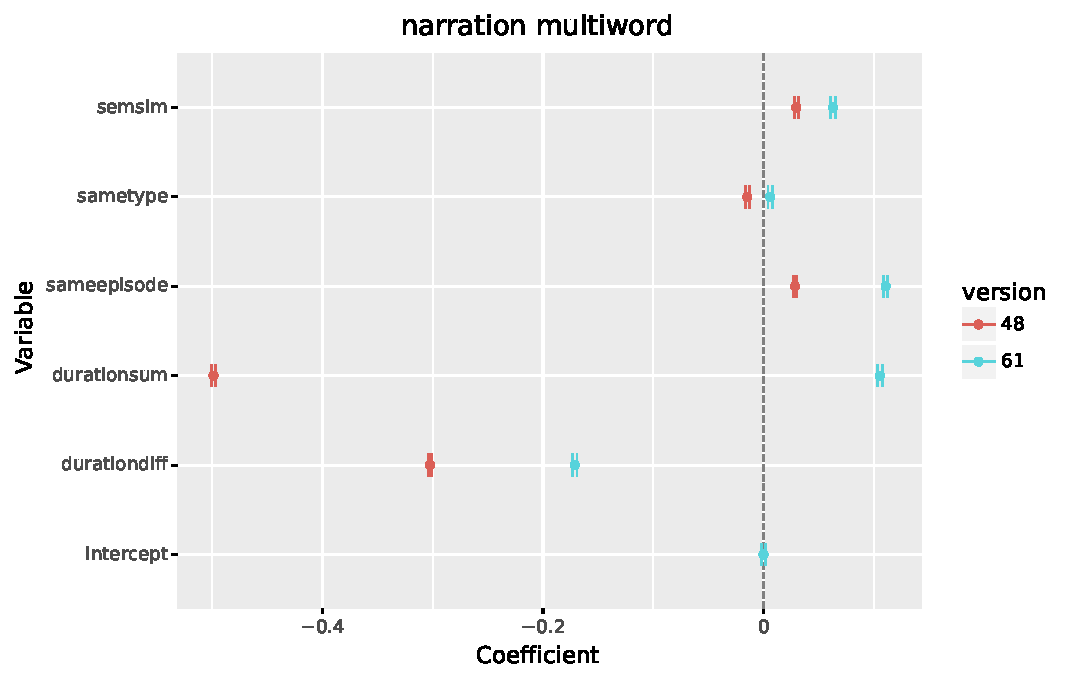
\includegraphics[scale=0.66]{results/grsa_narration_multiword_coef.pdf}
  \caption{Association of predictors with 
    model-based pairwise similarity scores for multi-word utterances
    in the narration validation data. Coefficients are standardized.}
  \label{fig:coef_multiword_narration}
\end{figure}


\todo{Update discussion of results}

%For both data subsets (dialog and narration), the highest magnitude
%predictors are {\tt durationdiff}, {\tt durationsum} and {\tt semsim}. The effect of
%the {\tt samespeaker} predictor for the dialog data is close to zero.
%These effect are there already for the pre-trained-only
%representations, but are strengthened for the fully-trained target
%model.  This results indicate that the model learns some aspects of
%word-level semantics as captured by GloVe word vectors, and that
%speaker identity does not appear to be a substantial impact on
%utterance embeddings.

The strength of the association between effects of utterance
duration {\tt durationdiff}, {\tt durationsum} and pairwise similarities apparent in this
data was suprising and possibly undesirable. We conjecture that is
arises as an effect of the positional encodings in the transformer
layers.

\begin{table}
  \centering
  \begin{adjustbox}{angle=90}
    \begin{tabular}{lrrrrrrrr}
\toprule
{} &  samespeaker &  sameepisode &  sametype &  glovesim &  distance &  durationdiff &  similarity &  similarity\_init \\
\midrule
samespeaker     &         1.00 &         0.21 &      0.01 &      0.02 &     -0.01 &          0.01 &       -0.00 &             0.02 \\
sameepisode     &         0.21 &         1.00 &      0.02 &      0.02 &     -0.01 &          0.00 &        0.02 &             0.03 \\
sametype        &         0.01 &         0.02 &      1.00 &      0.22 &     -0.48 &         -0.03 &        0.03 &             0.02 \\
glovesim        &         0.02 &         0.02 &      0.22 &      1.00 &     -0.10 &         -0.16 &        0.16 &             0.12 \\
distance        &        -0.01 &        -0.01 &     -0.48 &     -0.10 &      1.00 &          0.00 &       -0.00 &            -0.01 \\
durationdiff    &         0.01 &         0.00 &     -0.03 &     -0.16 &      0.00 &          1.00 &       -0.63 &            -0.48 \\
similarity      &        -0.00 &         0.02 &      0.03 &      0.16 &     -0.00 &         -0.63 &        1.00 &             0.81 \\
similarity\_init &         0.02 &         0.03 &      0.02 &      0.12 &     -0.01 &         -0.48 &        0.81 &             1.00 \\
\bottomrule
\end{tabular}

  \end{adjustbox}
  \caption{Variable correlations, dialog pairwise similarity data.}
  \label{tab:dialogvarcor}
\end{table}
\begin{table}
  \centering
  \begin{adjustbox}{angle=90}
    \begin{tabular}{lrrrrrrr}
\toprule
{} &  sameepisode &  sametype &  glovesim &  distance &  durationdiff &  similarity &  similarity\_init \\
\midrule
sameepisode     &         1.00 &      0.01 &      0.01 &     -0.01 &         -0.00 &        0.02 &             0.02 \\
sametype        &         0.01 &      1.00 &      0.40 &     -0.61 &         -0.09 &        0.07 &             0.06 \\
glovesim        &         0.01 &      0.40 &      1.00 &     -0.28 &         -0.22 &        0.26 &             0.18 \\
distance        &        -0.01 &     -0.61 &     -0.28 &      1.00 &          0.07 &       -0.05 &            -0.05 \\
durationdiff    &        -0.00 &     -0.09 &     -0.22 &      0.07 &          1.00 &       -0.51 &            -0.41 \\
similarity      &         0.02 &      0.07 &      0.26 &     -0.05 &         -0.51 &        1.00 &             0.75 \\
similarity\_init &         0.02 &      0.06 &      0.18 &     -0.05 &         -0.41 &        0.75 &             1.00 \\
\bottomrule
\end{tabular}

  \end{adjustbox}
  \caption{Variable correlations, narration pairwise similarity data.}
  \label{tab:narrationvarcor}
\end{table}
